\hypertarget{index_intro}{}\section{Introduction}\label{index_intro}
The \char`\"{}Wi-\/11 Machine\char`\"{} is a simple, 16-\/bit computer architecture. It has 8 general purpose registers, 3 condition code registers (CCRs), and a program counter (PC). This software package is meant to emulate its execution, as well as present the user with information regarding the state of the machine after each instruction is executed. However, before one can delve into the behind-\/the-\/scenes details, one must understand the environment. In particular, an understanding of the object file syntax and the interactions between the components used in this project is necessary.\hypertarget{index_syntax}{}\section{Object Files}\label{index_syntax}
\begin{DoxyParagraph}{}
The object files (ususally file\_\-name.o) that this simulator accepts are ascii text files with the following structure: \begin{DoxyItemize}
\item One \hyperlink{index_header}{Header Record} \item Several \hyperlink{index_text}{Text Records} \item One \hyperlink{index_end}{End Record}\end{DoxyItemize}

\end{DoxyParagraph}
\hypertarget{index_header}{}\subsection{The Header Record}\label{index_header}
\begin{DoxyParagraph}{}
The Header Record is a single line that prepares the system for the storing the instructions to come. 
\end{DoxyParagraph}
\begin{DoxyParagraph}{}
{\bfseries Components} \begin{DoxyItemize}
\item A capital 'H'. This designates that it is the Header Record. \item A 6 character \char`\"{}segment name\char`\"{} (anything will do). \item A 4-\/digit Hexadecimal value that corresponds to the \char`\"{}load address\char`\"{} of the program. Instructions can be written starting at this address. \item A second 4-\/digit Hexadecimal value that denotes the length of the program-\/load segment (the size of memory into which the instructions will be loaded). \end{DoxyItemize}

\end{DoxyParagraph}
\begin{DoxyParagraph}{}
{\bfseries At a glance:} There is an 'H', a segment name, the first location where instructions can be written, and the number of memory locations for instuctions.
\end{DoxyParagraph}
\hypertarget{index_text}{}\subsection{Text Records}\label{index_text}
\begin{DoxyParagraph}{}
Following the Header Record are serveral Text Records. Each Text Record corresponds to a single machine instruction and, like the header record, is on a single line. 
\end{DoxyParagraph}
\begin{DoxyParagraph}{}
{\bfseries Components} \begin{DoxyItemize}
\item A capital 'T'. This designates that it is a Text Record. \item A 4-\/digit hexadecimal value -\/-\/ The location in memory at which the instruction will be stored. \item A second 4-\/digit Hexadecimal value -\/-\/ The encoding of the instruction to be stored. \end{DoxyItemize}

\end{DoxyParagraph}
\begin{DoxyParagraph}{}
{\bfseries At a glance:} There is a 'T', the location to store the instruction, and the instruction itself.
\end{DoxyParagraph}
\hypertarget{index_end}{}\subsection{The End Record}\label{index_end}
\begin{DoxyParagraph}{}
The End Record is, as the name would suggest, the last line of the line. Its purpose is to denote the end of instructions to be written and to give an initial value for the PC.\par
\par
 
\end{DoxyParagraph}
\begin{DoxyParagraph}{}
{\bfseries Components} \begin{DoxyItemize}
\item The End Record begins with a capital 'E'.\par
 \item Next, and last, a 4-\/digit hexadecimal value to be put into the PC. \end{DoxyItemize}

\end{DoxyParagraph}
\begin{DoxyParagraph}{}
{\bfseries At a glance:} There is an 'E', and the location in memory from which the first instruction should be fetched.
\end{DoxyParagraph}
\hypertarget{index_Component}{}\section{Interaction}\label{index_Component}

\begin{DoxyImageNoCaption}
  \mbox{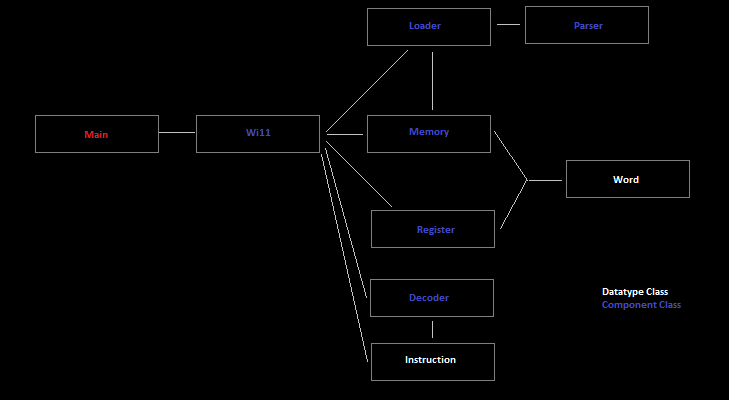
\includegraphics[width=\textwidth]{software_interaction.png}}
\end{DoxyImageNoCaption}
 \hypertarget{index_components}{}\subsection{Components}\label{index_components}
\hypertarget{index_instructions}{}\subsection{Wi11 Instruction Set}\label{index_instructions}
